\documentclass[letterpaper,11pt]{article}

\usepackage{graphics,graphicx, amsmath, amssymb,xcolor}
\usepackage{txfonts} 
\usepackage{balance}
\usepackage[sort&compress]{natbib}
\usepackage{hyperref}

\setlength{\textwidth}{6.5in} 
\setlength{\textheight}{9in}
\setlength{\topmargin}{-0.0625in} 
\setlength{\oddsidemargin}{0in}
\setlength{\evensidemargin}{0in} 
\setlength{\headheight}{0in}
\setlength{\headsep}{0in} 
\setlength{\hoffset}{0in}
\setlength{\voffset}{0in}

%\makeatletter
%\renewcommand{\section}{\@startsection%
%{section}{1}{0mm}{-\baselineskip}%
%{0.5\baselineskip}{\normalfont\bfseries}}%
%\makeatother

\newcommand{\no}{\noindent}
\newcommand{\comment}[1]{{\color{red}\bf{(#1)}}}

\def\apj{ApJ}
\def\apjl{ApJ}
\def\apjs{ApJ}
\def\mnras{MNRAS}
\def\pasj{PASJ}
\def\aap{A\&A}
\def\prd{Phys. Rev. D.}
\def\araa{ARAA}
\def\nat{Nature}

\begin{document}
\pagestyle{plain}
\pagenumbering{arabic}

\begin{center} 
\Large\bfseries{Simulating Cosmic Weather in Galaxy Clusters and Groups with XSEDE}
\end{center}

\begin{center}
PI: Daisuke Nagai \\
Co-PI: Erwin Lau
\end{center}

\medskip
\centerline{ \large \bf Abstract}
We request a new research allocation to run high resolution cosmological simulations of formation galaxy clusters and groups. We aim to understand the how the physical properties of galaxy clusters and groups are shaped by  ``cosmic weather'' events, i.e., mergers with other galaxies and groups, and accretion from large-scale filaments. In particular, we would like to understand how the highly non-linear coupling between the large-scale ``cosmic weather'' and the small-scale active galactic nuclei (AGN) feedback physics can explain multi-phase gas properties in the cores of clusters and groups in recent state-of-the-art galaxy cluster observations from the {\em Chandra} and {\em Hitomi} X-ray observatories, the {\em Hubble} Space Telescope, and from microwave observations with ALMA. Due to the multi-scale nature of the problem, the computing resources at XSEDE (in particular the latest Skylake nodes deployed at Stampede2) will enable us to perform unprecedented high resolution simulations of galaxy clusters and groups that will cover the large-scale cosmic weather physics and small-scale AGN feedback physics. the two main processes that governs the properties of gas in galaxy cluster cores. Outputs of the proposed simulation will be used to develop effective subgrid model of AGN feedback physics that can be applied to inexpensive, coarse resolution all-sky simulations, which are crucial for constraining cosmological parameters with upcoming galaxy cluster surveys. 
%in the with the aim of understanding galaxy clusters astrophysics with unprecedented numerical resolution and realistic physical modeling. The proposed simulations follow the evolution of dark matter in a cosmological volume, with realistic astrophysics of star formation, radiative processes in the gas and feedback from active galactic nuclei and supernovae. In particular, we will compare three different models of active galactic feedback against the recent state-of-the-art galaxy cluster observations from the {\em Chandra} and {\em Hitomi} X-ray observatories. The AGN model best matching the observations will then be turned into a sub-grid prescription for upcoming all-sky volume simulations, which are crucial for making predictions for upcoming galaxy cluster surveys (such as {\em eROSITA}).
\medskip

\section{Scientific Background}
%Describe big picture of AGN feedback in galaxy and galaxy cluster formation: 
%Galaxy clusters play an important role in modern precision cosmology. As the most massive virialized objects in the universe, their abundance across cosmic time depends sensitively on the energy content of the universe, thus they provide exquisite constraints on cosmological parameters that are competitive and complementary to other cosmological probes. In the next decade, multi-wavelength cluster surveys (optical, X-ray, and microwave) will improve statistical constraints in cosmological parameters by detecting orders of magnitude more clusters.  Systematic uncertainties due to astrophysical processes during the formation of galaxy clusters will become dominant over statistical uncertainties in these cosmological constraints. The success of these cluster missions therefore depends critically on understanding and controlling systematic uncertainties due to cluster astrophysics. 

Galaxy clusters are powerful laboratories for studying astrophysics and cosmology. Their dense environments are suited for studying the physical processes responsible for galaxy evolution, such as ram pressure stripping and tidal effects. The weakly collisional intracluster medium (ICM) provides excellent laboratories for studying plasma physics, with implications for stellar winds and the interstellar medium \citep{Schekochihin2009}. As cosmological probes, the evolution of galaxy clusters clusters directly provides constraints in Dark Energy equation of state and amplitude of Dark Matter fluctuations, complementing other cosmological probes, such as cosmic microwave background, baryon acoustic oscillations, and supernovae Ia \citep{Planck2016}. 

%One of the biggest challenges of using clusters as effective astrophysics labs and cosmological probes is the lack of understanding of the physics of galaxy clusters, especially the behavior of the baryonic components (galaxies and gas) in the cluster core regions. 
One of the biggest challenges facing clusters astrophysics is to understand the role of physics of baryonic components (galaxies, and gas in the ICM), especially in the central regions of clusters, in shaping the observed  properties of galaxy clusters. The high density environment in the cluster cores means that radiative cooling (proportional to the square of gas density) becomes a runaway process, and needs heating mechanisms to regulate cooling to avoid excess star formation that are not observed. Feedback from the active galactic nuclei (AGN) residing in the centers of the brightest central galaxies in clusters, are believed to provide the energy required to offset cooling, however, the feedback mechanisms have not been fully understood. This leads to uncertainties in the thermodynamics of the cluster gas, introducing systematics in our ability to constrain cosmology with clusters at percent-level accuracies.  
%First, radiative cooling of gas is unstable as the cooling is proportional to the square of gas density. Cooler gas sinks closer to the center, where the density is even higher and so cooling even more efficient. Unless balanced by some heating mechanism, the runaway cooling would result in excess X-ray emission from the cooling gas and H-alpha emission from star formation, that are hundreds of times brighter than observed \citep{Nulsen1986}. Currently, feedback from active galactic nuclei (AGN) is the best candidate for regulating the the heating-cooling balance in cluster cores. Since X-ray luminosity profiles are used to compute cluster density profiles, and total X-ray luminosity and stellar mass are used to measure cluster mass, AGN feedback also introduces mass and redshift-dependent changes in cluster mass estimates. This hinders our ability to constrain cosmology with clusters at percent-level precision using the methods described above. 

Despite its importance, AGN feedback physics is still very poorly understood. It is currently impossible to directly observe the accretion disks of the supermassive black holes (SMBHs) that provide feedback either as heat or as mechanical outflows. Current limitation in computation does not allow us to simulate the range of scales of the accretion and feedback physics involved, from the sub-pc scale near the vicinty of the SMBH (close to the Schwarzschild Radius), the 100~kpc scales where the feedback energy is injected to the cluster gas.  %We are left instead to piece together the underlying processes by matching observations of quasars and kinetic jets associated with the AGN with idealized simulations of the regions surrounding the central black hole. 
Numerical modeling of AGN feedback in clusters thus requires the use of multi-scale simulations, with each successively coarser simulation linking the theoretical understanding from smaller scale physics to effective models at the next until they match the scales of observations.

Within the next decade, X-ray observations, such as the X-ray Imaging and Spectroscopy Mission (XRISM), {\em eROSITA}, {\em Athena} and possibly {\em Lynx},  together with other multi-wavelength observatories, such as HSC and LSST in the optical, and SPT-3G,  AdvACT, and ALMA in microwave/sub-mm,  will provide an extraordinary amount of exquisite observational data of galaxy clusters, making the next decade the golden time to study them. We aim to fill this crucial gap in the theoretical modeling of clusters in time to interpret this wealth of new data.

\subsection{Current Status: Recent Observations of Galaxy Clusters and Groups}

Recent X-ray observations of galaxy clusters have provided important clues to understanding AGN feedback physics. Despite its short lifetime, {\em Hitomi} was able to directly measure gas motions in the core of the Perseus Cluster via Doppler line shifts and broadening of X-ray emission lines with its high-spectral resolution calorimeter.  %(See Figure~\ref{fig:hitomi}). 
This first measurement of gas motions provide new constraints on the AGN feedback mechanism.  AGN feedback was originally thought to drive gas motions in the cluster core, which then dissipate and heat the ambient ICM.  While indirect estimates of turbulent gas motions (inferred from X-ray fluctuation analysis) suggested that turbulent dissipation can provide enough energy to offset radiative cooling \citep{Zhuravleva2017}, the observed velocities of 100-150km/s cannot keep up with the radiative cooling flows, as they are too slow in spreading the energy throughout the cluster cores \citep{Fabian2017}. The successor to {\em Hitomi}, XRISM, is expected to provide more direct gas motions measurements in clusters once it launches in 2021. 

In addition recent {\em Chandra}-XVP observations of mass-limited clusters provide constraints on AGN feedback across cosmic time \citep{McDonald2017,McDonald2014}. The {\em Chandra}-XVP sample consists of massive clusters ($M_{500c} > 3\times 10^{14} M_\odot$) across a wide range of redshifts ($0.3 < z <1.9$). They are selected via the Sunyaev-Zel'dovich (SZ) effects with the South Pole Telescope (SPT).  The sample has provided unprecedented insights into the thermodynamical and chemical structure and evolution of the X-ray emitting ICM since the earliest epoch of cluster formation %(See Figure~\ref{fig:chandra_spt}).
In particular, it demonstrated the lack of evolution of the so-called ``cool-core'' galaxy clusters -- galaxy clusters that have cool dense gas cores with AGN feedback actively regulating heating and cooling. It further showed that the density, temperature, entropy of these cool-cores are already set in place as early as $z \sim 1.7$, when the majority of these clusters are still forming. Such evolutionary trend has not been successfully explained yet. Similarly, mass-limited SZ-selected clusters from the {\em Planck} satellite shows that fraction of these cool-core clusters does not change with time \citep{Andrade-Santos2017,Rossetti2017}. It is important to understand the formation and (lack of) evolution of these cool-core clusters, as they are likely to be over-represented in upcoming X-ray cluster surveys (e.g., eROSITA) since they are much brighter than their non-cool-core counterparts, especially at high redshifts.  

%Mass-selected samples of galaxy clusters, compiled using Sunyaev-Zel'dovich (SZ) measurements with telescopes like {\em Planck} and the South Pole telescope (SPT), provides other interesting constraints on the cluster core properties. These observations focus on understanding the evolution of gas cores in galaxy clusters from their formation to the present time. As non-coo that non-cool-core fractions of $30-40\%$ depending on the criteria used to define them \citep{Andrade-Santos2017,Rossetti2017}. These numbers are biased high for flux-limited samples. In other words, for the same mass, cool cores are brighter than non-cool cores, which would introduce systematic errors in mass functions reconstructed from luminosity functions in upcoming X-ray surveys. 

Most existing simulations produce too many cool cores, with non-cool cores only formed in low angular momentum major mergers. Observations do not support a primarily merger-driven disruption of cool cores \citep{OHara2006}. Current state-of-the-art cosmological hydrodynamical simulations of galaxy clusters, such as Illustris-TNG \citep{Barnes2017b}, produces too many cool-core clusters at $z\geq 1$. There, the cool core disruption is feedback driven, but still begins too late and happens too rapidly, leading to mismatch with observations. Thus, it is necessary to develop an effective model that accurately capturing the both the effects of AGN feedback and mergers on cluster core thermodynamics, anticipating upcoming cluster surveys. 

We aim to develop a successful AGN sub-grid model that heats up the gas in the cores of clusters while maintaining low turbulent velocities, matching the observed  cool-core and non-cool-core cluster fractions since the formation of the earliest clusters at $z\sim 2$.

\subsection{Challenges in modeling AGN feedback physics: the Role of ``Cosmic Weather''}

The major challenge of modeling AGN feedback physics in galaxy clusters is the wide range of physical scales involved: from parsec (pc) scale in the accretion and feedback physics of supermassive blackholes (SMBH) to $\sim 100$~Mpc in modeling cluster formation in a cosmological context. Due to the lack of resolution, AGN feedback models in cosmological simulations must rely on heavily parametrized sub-grid models, which are difficult to constrain observationally or theoretically. As such, they are fine-tuned to match observations, which compromises the predictive power of the simulations. Due to insufficient resolution, cosmological simulations until recently implemented AGN feedback as injections of thermal energy. This does not reproduce the observed thermodynamic or kinematic properties in observed clusters \citep{Lau2017}. The artificially high cooling rates due to insufficient resolution means that large amounts of thermal energy need to be injected to match the observed gas and stellar mass fractions in clusters and groups, requiring unphysical feedback efficiencies from the AGN and resulting in overheated gas.

On the other hand, idealized simulations of isolated clusters, which offer much higher resolution ($\sim 100$~pc), are able to reproduce some of the observed cluster core properties. Besides the higher resolution, two aspects of the idealized prescriptions have been particularly successful - temperature-dependent accretion onto the black hole, which enforces a tighter feedback loop, and mechanical outflows, which push the reheated gas out of the dense core to prevent rapid overcooling \citep[e.g.,][]{Meece2015, Li2015}. In particular, the idealized simulations in \citet{Gaspari2015} drew black hole accretion rates from GR-RMHD simulations of the black hole vicinity, and prescribes a feedback efficiency as a function of the gas cooling rate so that the system is in thermal quasi-equilibrium by construction. The idealized simulations, however, require very large precession rates for the jets to distribute the feedback energy roughly isotropically. They also transfer most of their energy to the ICM via very strong shocks, which are not observed. 

The key limitation of idealized simulations is that they do not model ``cosmic weather'', i.e., the effects of large-scale structure growth such as accretion and mergers on the small-scale gas physics. Mergers and accretion can enhance the flow of low angular momentum gas into the core, seed turbulence on large scales which can bend the AGN jets without requiring precession at the source \citep{Tremmel2018} %(See Figure~\ref{fig:RomulusC}).
and mix the cluster gas, aiding the transport of heat and metals from the highly enriched central gas. While mechanical outflows have been the most successful feedback model in idealized simulations, tests have shown that most of the effects of kinetic feedback can be approximated by temporarily shutting of cooling in the cells receiving thermal feedback \citep{Smith2017} or by injecting thermal energy at different radii at different times \citep{Vazza2013}. To make progress, it is necessary to compare these various effective AGN feedback models to observations, and identify physically motivated values for any of the free parameters.

We propose a pilot simulation program to bridge the gap between the high-resolution idealized simulations and the low-resolution cosmological simulations with a multi-scale approach of modeling ``cosmic weather'' in galaxy clusters and groups. We will perform cosmological simulations of galaxy cluster with unprecedented high numerical resolution comparable to the coarsest idealized simulations, which have already been tested for convergence with their higher resolution counterparts. We will progressively coarsen the resolution to identify modifications needed for ever larger volume simulations. 
This allow to systematically understand the effects of resolution on the subgrid AGN physics module, which is complementary to the latest high resolution idealized and cosmological simulations. 
The results of the proposed simulations will enable us to construct effective, physical sub-grid AGN feedback models for very large volume hydrodynamic simulations ($\geq 1$~Gpc), and semi-analytic models for all-sky dark matter-only simulations, which are required to improve the cosmological constraints derived from upcoming surveys of the galaxy groups and clusters.
%The proposed simulation project will advance our understanding of the formation of galaxy clusters and groups from the observable emission from their gas and stellar content, which 
\section{Research Goals}

Our primary science goal is to understand the interplay between AGN feedback physics in galaxy clusters and groups, and the ``cosmic weather'' of mergers and accretion, and assess their impact on the structure and evolution of the ICM as well as the use of galaxy clusters and groups as cosmological probe. We propose to use multi-scale hydrodynamical cosmological simulations which will address the following outstanding issues in galaxy clusters astrophysics: 

\begin{itemize}

\item Understand and constrain AGN feedback models in the cosmological context, by comparing outputs of our cosmological simulations to state-of-the-art observations of clusters and groups. Specifically, we will distinguish different SMBH accretion models (Bondi versus cold chaotic accretion -- described in Section~\ref{sec:agn}) and feedback models (thermal versus kinetic) via detailed comparisons in the thermal, kinematic and chemical properties between model predictions and observations. 

\item Understand the nature and origin of gas motions in galaxy clusters (AGN feedback versus cosmic accretion such as mergers), and their roles in thermal heating and cooling balance.  
Specifically, this will help interpret/resolve the apparent discrepancy between the direct measurement of turbulence with {\em Hitomi} in the Perseus cluster and the surface brightness fluctuation analysis from the {\em Chandra} measurements. 

\item Understand the effects of substructure accretion and feedback on the gas properties in cluster outskirts. Specifically, this will shed light on the physical processes (feedback versus ram pressure stripping) responsible for the chemical enrichment in the ICM and the nature of gas inhomogeneities (gas clumping) in the virialization region in the outskirts of galaxy clusters and groups. 

\item Understand nature and evolution of the global properties of the ICM across cosmic time, from the epoch of cluster formation ($z \sim 2$) to the present time, and build models to account for such evolution. This will allow us to control astrophysical uncertainties in cluster-based cosmological constraints associated with galaxy cluster mass estimates, observable-mass scaling relations, and cluster selection functions in the cosmological constraints in upcoming galaxy cluster surveys. 

\end{itemize}

%\section{Research Questions}
%\subsection{Constraining AGN Feedback Physics with Simulations and Observations.}
%The biggest mystery in AGN feedback is how the feedback energy couples with the cluster gas. There are three possible physical processes via which the AGN can heat the gas: through weak shocks or sound waves excited from the AGN jet/bubble; through turbulent dissipation of the AGN-driven gas motions; or through mixing of the hot plasma in the AGN bubble with the surrounding ICM. All three processes are expected to play different roles throughout the AGN feedback cycle, but their relative importance is not understood. 

%The recent {\em Hitomi} observations of the Perseus cluster suggested a promising way to understand AGN heating. These observations showed fairly uniform ICM properties with little variations in velocity, density, temperature, and metal abundances throughout the cluster cores across the resolution element of the calorimeter onboard.  The high spectral resolution of {\em Hitomi} was able to detect inhomogeneities along the line of sight, by measuring any deviation from the Gaussian emission line shape. The close-to-Gaussian shape of the emission line observed in the Perseus core already rules out models of AGN feedback that create too much ICM fluctuations (such as thermal blastwave feedback).  The ``gentle'' kinetic AGN feedback, on the other-hand, seems to be consistent with observations \citep{lau_etal17}.  

%To pin down the specific mechanisms for AGN heating at the different stages of AGN feedback, we need to predict the observational signatures in the ICM fluctuations generated by these heating processes, which can then be probed by current and upcoming X-ray observations. We also need to account for fluctuations that are not generated by AGN feedback. Cosmic accretion, such as mergers, can bring gaseous substructures near the line-of-sights to the cluster cores. These gas substructures, mostly likely associated with infalling groups and galaxies, can create apparent fluctuations in the ICM that have nothing to do with AGN feedback. In addition, infalling groups can generate turbulence, which create additional ICM fluctuations. 
 
%Our ultra-high resolution cosmological simulations implemented with physical AGN feedback models are ideal for making predictions for observations of ICM fluctuations.  First, our cosmological simulations with AGN feedback are ideal for disentangling the ICM fluctuations due to AGN feedback from cosmic accretion.  Second, our mock X-ray pipeline allows us to generate realistic X-ray maps and spectra for identifying robust observational signatures of different AGN heating processes through the comparisons between simulations and observations. 

%First constraints on AGN feedback physics can be made by comparing our simulations with the existing {\em Hitomi} observations, which already provides exquisite data on the thermodynamical, kinetic, and chemical structures in the core of the Perseus cluster. The results will also pave the road for the planning of the observational missions in the coming years. 
%\subsection{Explaining the Origins of Cool Core and Non-cool Core Clusters.}
%Closely related to AGN feedback physics is the the so-called cool core/non-cool-core problem in galaxy clusters. It refers to the two apparently distinct populations of galaxy clusters: ``cool core (CC)'' clusters with low gas entropy cores,  and ``non-cool core (NCC)'' clusters with high gas entropy core. It is important to understand the fraction of CC and NCC clusters with redshifts to control for any selection biases in upcoming X-ray cluster surveys, since CC clusters are more X-ray bright. 

%It remains unclear how these cool-cores are formed, maintained, and destroyed during the evolution of the cluster -- whether it is due to baryonic physics such as AGN feedback physics, or the cluster mass accretion history such as major mergers. Understanding the origin of the core variation is important for understanding galaxy cluster formation and evolution, and for understanding how clusters are selected for constraining cosmology. Previous simulations have limited success in understanding the cool-core/non-cool-core variations: isolated idealized simulations do not model the accretion history of the cluster; while cosmological simulations lack physical AGN feedback models. We need to model both AGN feedback and cosmic accretion self-consistently to tackle this problem. 

%Our ultra-high resolution simulation with physical AGN feedback model are suitable for solving the CC/NCC problem.  The comparison of our ultra-high resolution cosmological simulations against existing X-ray observations of well-known CC (e.g., Perseus) and NCC clusters (e.g., Coma) (with {\em Suzaku}, {\em Hitomi}, and {\em Chandra}) will allow us to constrain both the AGN physics in the cluster core, and accretion histories with cluster outskirts. While the larger statistical samples of simulated clusters will characterize the fraction of CC/NCC clusters across cosmic time. This will shed light on the different physical processes (AGN versus cosmic accretion) that give rise to the evolution of CC/NCC cluster populations. 

%The results from this comparison will anchor our understanding of cluster scaling relations, serving as a baseline result for shedding light on the evolution of the scaling relations at higher redshift which are important for probing dark energy with evolution in cluster abundance. 

\section{Computational Case}
%\section{Resource Usage Plan}
\subsection{Cosmological Simulation with ART}\label{sec:art}

The proposed cosmological simulations will be performed with the Adaptive Refinement Tree ({ART}) code \citep{kra99,kra02,rudd_etal08}, an adaptive mesh refinement (AMR) $N$-body and hydrodynamical code that follow structure formation in the cosmological context. 
As an Eulerian code, ART can accurately model the key thermodynamical and kinematic processes (e.g., shocks, entropy, and turbulence) in the ICM. In addition, the adaptive nature of ART allows for a high dynamic range of $\geq 10^9$, capable of reaching high mass and spatial resolution necessary for resolving the small-scale AGN feedback physics in the cores of clusters and groups. 

The current {ART} code is equipped with a variety of subgrid models for modeling baryonic physics (including radiative gas cooling, star formation, and energy feedback from stars that are important for detailed modeling of the stellar distributions in cluster galaxies. We have developed a thermal AGN feedback module for the {ART} code discussed below \citep[also see][for the first implementation of AGN feedback into the {ART} code]{nagai_etal13}. The left panel of Figure~\ref{fig:sims} shows the total baryon, gas, and stellar fraction for the {\em Omega500} simulation \citep{nelson_etal14} with different baryonic physics, including a run with the thermal AGN feedback model. 

The ART code is equipped with two major analysis modules which are essential for getting meaningful insights from the comparison with observations. Its mock X-ray pipeline generates synthetic X-ray photon maps and spectra of galaxy clusters convolved with the instrumental responses,  allowing us to make direct and meaningful comparisons between simulations and observations form {\em Suzaku}, {\em Hitomi}, and the future XRISM mission.  The right panel in Figure~\ref{fig:sims} shows an example mock X-ray map from one of our cosmologically simulated clusters.  The ART code is also equipped with a merger tree code that gives us the full formation history of individual galaxy clusters by tracking cluster mergers across different epoch, which is needed for studying the effects of mergers on ICM properties, and the interplay between mergers and AGN feedback. 

\begin{figure}[t]
\centering
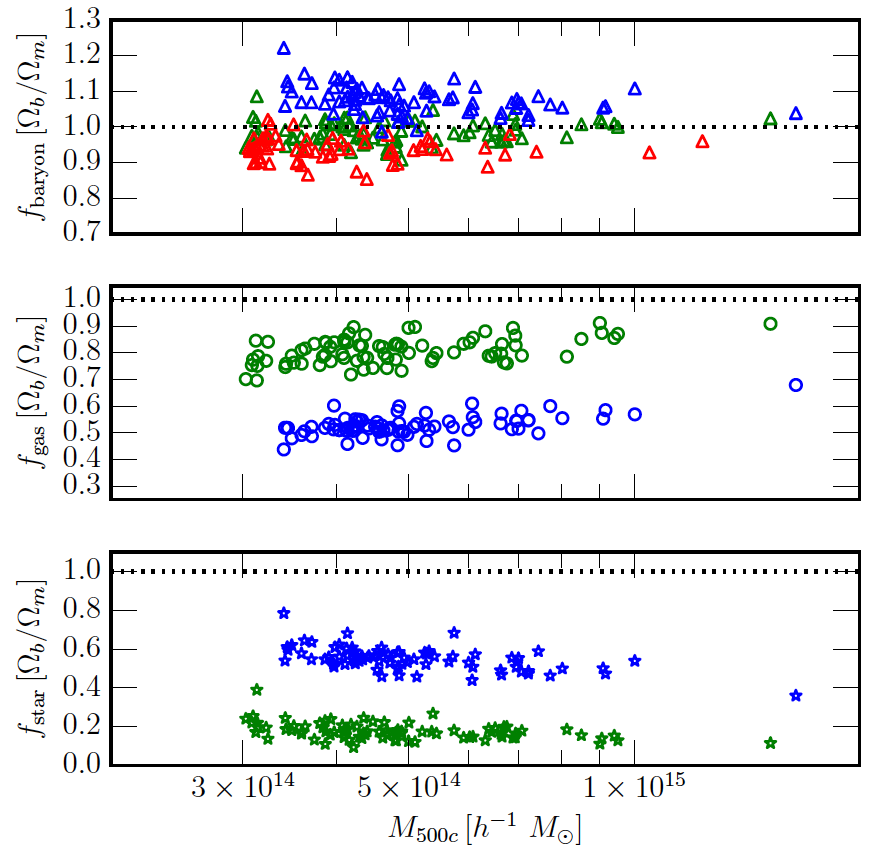
\includegraphics[width=0.40\textwidth]{fbaryon.png}\;\;\;\;
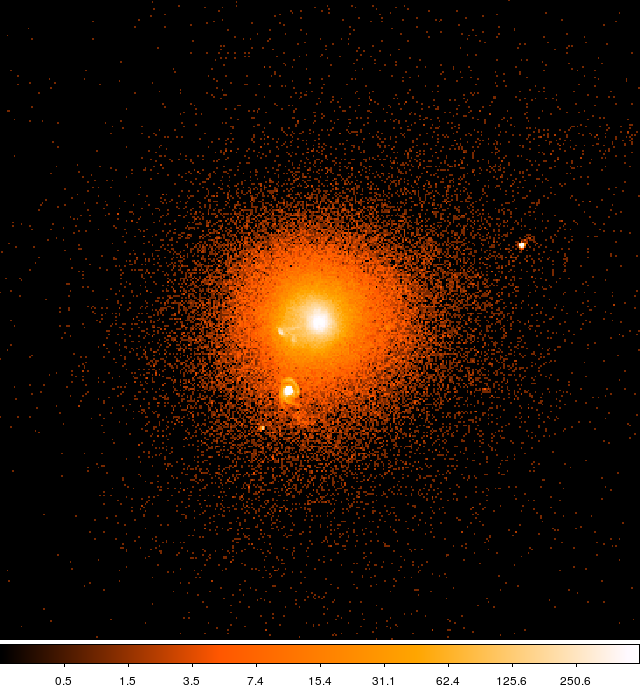
\includegraphics[width=0.35\textwidth]{mock_chandra.png}
\caption{
{\em Left}: Baryon, gas, and stellar fraction (top, middle, bottom panels respectively) of the {\em Omega500} simulations, showing the runs with non-radiative physics (red points), with radiative cooling, star formation, and supernova feedback (blue points), with the addition of thermal AGN feedback on top of radiative cooling, star formation, and supernova feedback (green points).  
{\em Right}: Mock X-ray map of our simulated cluster with thermal AGN feedback at $0.1-10$~keV, observed for $10$~ks at a redshift of $0.06$. }  
\label{fig:sims}
\end{figure}

\subsection{AGN Feedback Modules}\label{sec:agn}

One of the key science objectives is to understand the influence of mergers and accretion on AGN feedback, and to develop effective subgrid AGN feedback models for large-scale cosmological simulations. To this end, we will simulate two AGN feedback modules: thermal AGN feedback (tAGN) and kinetic AGN feedback (kAGN). The tAGN feedback model has been widely adopted in the current generation of cosmological simulations. Our simulation with tAGN will serve as a reference AGN feedback simulation for us to compare against our novel kinetic AGN feedback module. 

The ART code already has a working tAGN module. In this module, we follow the accretion and mergers of BH in dark matter halos as in \citet{booth_schaye09}. The BH particles are first seeded with an initial mass of $10^5h^{-1}M_\odot$ at the centers of resolved dark matter halos. As the simulation progresses, these BH particles accrete gas with a rate given by a modified Bondi accretion model and return the feedback energy as a fraction of the accreted rest mass energy into the environment in the form of thermal energy.  To keep the thermal feedback from the BH from immediately radiating away, following \citet{booth_schaye09} we require that the BH stores enough feedback energy until it accumulates enough energy to heat neighboring gas cells by at least $10^7$~K. However, this way of injecting thermal energy to the gas fails to account for thermodynamic, kinetic, and chemical properties observed in the cores of galaxy clusters. 

The main challenge here is the short radiative cooling time of the gas, compared to the numerical resolution of cosmological simulations, meaning that the cooling process are not properly resolved. Recent high resolution cosmological simulations shows that shutting off cooling temporarily can mitigate this problem and produce gas cores that matches observations \citep{Tremmel2018}. 

Alternatively, instead of heating the ICM by directly injecting thermal energy from the AGN, one can instead inject kinetic energy and momentum from the AGN. In this way,  build-up of dense gas cores is prevented by displacing dense gas from the cores; at the same time the ICM around the cluster core is heated more gently via dissipation and mixing by the gas motions injected by the AGN, compared to the unphysical ``thermal bomb'' in the conventional thermal AGN feedback models. One of the more promising models of kinetic AGN feedback is the so-called ``cold chaotic accretion''  \citep[CCA,][]{gaspari_etal13} or the ``precipitation'' model \citep{voit2018}, in which gas are uplifted from the cluster center to the outer regions by AGN outflow, becomes thermally unstable and condenses into a colder dense phase, and eventually accreted chaotically into the SMBH that fuels the outflow, forming a natural AGN feeding and feedback cycle. There are observational evidence for model by recent observations \citep[e.g.,][]{tremblay_etal16}, which revealed reservoirs of thermally unstable gas in the cluster cores. 
%There has been a number of developments on improving the physicality of AGN feedback modules. One of the more promising ones is the recently proposed subgrid kinetic AGN feedback model by \citet{gs17}. The attractive feature of this model is that it addresses the wide range scales in AGN feedback: from near the Schwarzschild radius of the BH ($\sim$~pc), to the radial extent of the massive cluster galaxies $\sim 100$~kpc, by calibration from high-resolution hydrodynamical simulations of AGN feedback, as well as magnetohydrodynamic simulations of SMBH accretion with general relativity. This model is supported in part by recent ALMA observations \citep{tremblay_etal16}, which revealed reservoirs of condensed cold gas due to thermally unstable gas in the cluster cores. The cold gas fuels the SMBH and power AGN feedback on the surrounding ICM. This picture is also supported by observations of cold dense filamentary structures seen in the core of the Perseus cluster.  
%The kAGN module will be available by the time the computing resources are allocated. 

In our proposed simulations program will explored these new ways of improving the physicality of AGN feedback in cosmological simulations. Specifically, we will run two versions of AGN feedback physics:  thermal AGN feedback (tAGN) with cooling shut-off, 
%(2) thermal AGN feedback with cooling shut-off (tAGN-NOCOOL), 
and kinetic AGN feedback (kAGN), where we will systematically compare their impact on the physical properties of cores in galaxy groups and clusters. By assessing their dependence on numerical resolution, we will also develop effective subgrid AGN feedback modules for large-scale cosmological simulations. 

\subsubsection{Proposed Simulations}

\begin{table}[t]
\centering
\begin{tabular}{l c c c c c }
Name & Box size & $\Delta x$ & $m_{\rm DM}$ & $N_p$  \\
& [$h^{-1}$Mpc] & [$h^{-1}$kpc] & $[h^{-1}M_\odot] $ \\
\hline
\hline
%HR $\times 2$ & 50.0 & 0.27 & $1.5\times 10^5$ & $4096^3$  \\
HR $\times 2$& 50.0 & 0.54 & $1.2\times 10^6$ & $2048^3$ \\
LR $\times 2$& 50.0 & 1.08 & $9.6\times 10^6$ & $1024^3$ \\
\hline
%L100HR $\times 3$ & 100.0 & 0.54 & $1.2\times 10^6$ & $4096^3$ \\
%L100MR $\times 3$ & 100.0 & 1.08 & $9.6\times 10^6$ & $2048^3$  \\
%L100LR $\times 3$ & 100.0 & 2.16 & $1.9\times 10^7$ & $1024^3$ \\
\hline
\label{tab:sims}
\end{tabular}
\caption{Proposed Simulation Runs. The simulation box will have two physics runs, one with the thermal AGN feedback module, the thermal AGN feedback module with cooling shut-off, and the kinetic AGN feedback module.  $\Delta x$ is the finest spatial resolution, $m_{\rm DM}$ is the mass of the finest resolution dark matter (DM) particle, and $N_p$ is the effective number of DM particles of the simulation run. }
\end{table}

%Smaller, less massive halo have shallower gravitational well, the effects of AGN feedback depends on halo mass. Thus in order to develop a {\em consistent} AGN feedback modules for both group- and cluster-scale halos. Thus, we propose to simulate two boxes:(1) L50 Box with computational volume of $(50 h^{-1}{\rm Mpc})^3$ to simulate a massive group with mass $5 \times 10^{13} h^{-1}M_\odot$, and a (2) L100 Box with computational volume of $(100 h^{-1}{\rm Mpc})^3$ for cluster with mass $3\times 10^{14}h^{-1}M_\odot$. 

We propose to run our galaxy cluster cosmological simulations with unprecedented high numerical resolutions. The high spatial resolution is necessary to develop and validate {\em effective} sub-grid models of AGN feedback in cosmological simulations through direct comparisons with idealized simulations with similar resolution. 
For the high resolution runs, the spatial resolutions will be $0.54 h^{-1}{\rm kpc}$, and mass resolution with dark matter particle mass of $m_{\rm DM} = 1.2 \times 10^6 h^{-1}M_\odot$ , reaching those of existing idealized simulations. As it is computationally expensive to achieve high mass resolution everywhere throughout the entire simulation volume, all of our proposed simulations will be ``zoomed-in'' simulations, where only the computational volume surrounding the group and cluster halos (typically a sphere centered on the halo with radius about 3 times the virial radius of the halo) will be populated with finest mass resolution particles. The mass of the dark particle in the HR simulation corresponds to and effective number of particles of $N_p=2048^3$. 

%For the high resolution runs of the L50 and L100 boxes, L50HR and L100HR, the spatial resolutions will be $0.27 h^{-1}{\rm kpc}$ and $0.54 h^{-1}{\rm kpc}$ respectively, matching those of existing idealized simulations. To reach such high spatial resolution, they will have very high mass resolution with dark matter particle mass of $m_{\rm DM} = 1.5 \times 10^5 h^{-1}M_\odot$ and $1.2 \times 10^6 h^{-1}M_\odot$ for L50HR and L100HR respectively. As it is computationally expensive to achieve high mass resolution everywhere throughout the entire simulation volume, all of our proposed simulations will be ``zoomed-in'' simulations, where only the computational volume surrounding the group and cluster halos (typically a sphere centered on the halo with radius about 3 times the virial radius of the halo) will be populated with finest mass resolution particles. The mass of the dark particle in the HR simulation corresponds to and effective number of particles of $N_p=4096^3$. 

To study the effects of resolution on the implemented AGN physics, we also propose to re-run the simulation at lower resolution with effective number of particles of $N_p=1024^3$, labeled as ``LR'' run.  These lower resolution simulations are necessary to assess the dependence of the AGN feedback physics on resolution for developing and calibrating effective subgrid AGN feedback module. 

To effectively compare the results of our simulations to existing high-quality, state-of-the-art observations of galaxy groups and clusters in the local universe from {\em Chandra} and {\em Hitomi}, our simulations will be run all the way to the present time at $z=0$. Table~1 summarizes the proposed simulation runs. 

\section{Justification of Resources}

To run the proposed simulations listed in Table~1, we request SU on Skylake nodes on Stampede2. We provide the justification of the requested SUs below, based on the test results detailed in the Code Performance and Scaling document. 
%The high resolution of the spatial resolution of the proposed simulations means that the each computation time step is small, which requires significant amount of computing resources. 

First, we request Skylake (SKX) nodes instead of nights Landing (KNL) nodes based on the performance test done on both types of nodes. Our MPI-OpenMP simulation performed $4-5$ times faster on SKX nodes than KNL nodes regardless of the number of MPI tasks and OpenMP threads.

Based on the test LR run (with $N_p = 1024^3$) performed on the SKX nodes on Stampede2, the total wall time for a single LR run is estimated around $10^4$ hours with 4 SKX nodes, or 40k SU. This estimate has taken into consideration that wall time for each time step increases as spatial resolution increases at late times. 
%To estimate the total CPU time needed to run the HR simulation, we use the $N_p = 512^3$ run completed to $z=0$ on our local machine. It takes about 200 core-hours for the simulation to advance to step 50, and 200k core-hours to finish the simulation at $z=0$ with 620 steps. For $N_p = 1024^3$, the simulation will take twice as much, i.e. 400 core hours to advance to step 50, and 400k core-hours to complete on our local machine. 
%As the time taken for each time step increases with time step due to the increase in the load in both hydro solver and gravity solver as hydro cell and inter-particle separation decrease in size.  
%We ran a test LR run with $N_p = 1024^3$ on Stampede2 with 4 SKX nodes, using the optimal configuration of 16 MPI task per node and 6 OMP threads per task . It takes approximately 15 minutes on 4 nodes (or 1 SU) to advance to step 50. Thus we estimate that it will take around $10k$~SUs to finish the LR run. 

For the MR run (with $N_p = 2048^3$), the mass resolution is increased by a factor of 8. This increases the total time by a factor of 8. In addition, based on our weak scaling test, there is $10\%$ increase in wall time when we increase the number of particles per core by a factor of 8. Thus we estimate it will take a total of 352k SU for each MR run. Similarly, the estimated SU for each HR run ($N_p = 4096^3$) is 3100k.

We proposed to run HR, MR, and LR runs, for each of the two AGN feedback models. Thus we estimate the total SU for running the two sets (L100 and L50 of simulations is ${\rm (40k+352k+3100k)\times  2 = 6984k}$. We also request additional $30\%$ SU for analyses (such as halo finding) that can only be performed on Stampede2, which resulted in total SU of ${\rm 6984\times 1.3 = 9079k}$. {\bf Thus we request a total of 9.1M SU for the SKX nodes on Stampede2.} 

For reference, we also provide estimates for the minimum number of requested SKX nodes needed at run time for each of our runs. The minimum number of nodes is determined by the size and resolution of the simulation. Each HR run (with $N_p = 4096^3$) requires total amount of memory of $2.4$~TB, meaning that we need at least 128 SKX nodes (with $192$~GB memory per node) in order to run the HR simulation. The total number of 128 SKX nodes available on the skx-normal queue on Stampede2 should be able to accommodate the nodes needed for each HR run. For each MR run ($N_p = 2048^3$) requires 8 time less nodes, at 16 SKX nodes, and each LR run ($N_p = 1024^3$) requires 2 SKX nodes. 

In addition to SU, we also request storage for our simulations. To follow the formation of the groups and clusters, in particular to identify time when mergers happen, we will need to store multiple simulation snapshots (include both particle and gas data). We plan to store $\sim 50$ snap shots per simulation following the formation of the cluster/group from high redshift $z=3$ to the present time at $z=0$. The number of snapshots are required to ensure that the mass assembly history of the cluster/group is tracked robustly. This will require approximately 1 TB, 8 TB and 64 TB for each of the LR, MR, and HR runs respectively. Thus, for the L50 and L100 boxes, each with three runs, we request total storage space of $(1+8+64)\times2\times3$ = 438 TB. 

\section{Other Computing Resources}

%We currently have access to 128 nodes on the {\em Omega} machine at Yale University. Each node houses Intel Xeon X5560 at $2.80$~GHz with 32 GB of memory. The machine will retire by the end of 2018. Until then, it will be used for code development purpose. 

We have access to the {\em Grace} machine at Yale, shared among all faculties and staff of the Graduate School of Arts and Sciences at Yale. {\em Grace} is equipped with Intel Xeon E5-2660 nodes with 20-28 cores and 120-250~GB of memory each. The clock speed for each core ranges from $2.0$~GHz to $2.6$~GHz, which is slower than the SKX nodes on Stampede2. In addition, the slow interconnection speed between nodes in {\em Grace} means that it is not optimized for proposed simulations which rely heavily on MPI-parallelization for performance. {\em Grace} will only be used for testing analysis code and pipelines for the proposed simulation. 
Thus, the requested SKX nodes on Stampede2 will be essential for running and analyzing the proposed simulations.

\section{Team Qualification}
PI Daisuke Nagai is an associate professor at Yale University. He is an expert on computational cosmology, with focus on galaxy clusters. He has overall responsibility for carrying out the research in this proposal,
mentoring of a graduate student, facilitating collaborations,
overseeing timely publications.
%He implemented most of the baryonic physics module (star formation, supernova feedback) in the ART code for the proposed run. His major role is to steer the scientific directions of the proposed project. 
His 3rd year PhD student Ms. Urmila Chadayammuri will be responsible for implementing the new AGN feedback physics module and running the proposed simulation.    
Co-PI Erwin Lau is currently a postdoc at the University of Miami. Prior to that he was an associate research scientist at Yale University with the PI. He has worked on analyzing cosmological simulations performed with ART. He will be working closely with Ms. Chadayammuri to implement the AGN feedback module and analyzing the outputs of the proposed simulations.

\bibliographystyle{apj}
\bibliography{references}

\end{document}

%%%%%%%%%%%%%%%%%%%%%%%%%%%%%%%%%%%%%%%%%%%%%%%%%%%%%%%%%
\newpage
\setlength{\parskip}{2mm}
% set the following commands into the bbl file
\setlength{\baselineskip}{5.5mm}

%\vspace{2mm}
\centerline{\bf \Large Daisuke Nagai}

\vspace{2mm} \noindent 
{\bf 1. Professional Preparation}

\vspace{1mm} \noindent
University of Michigan  \hspace{4.1cm}  Physics \& Mathematics \hspace{1.5cm} B.S. 1999 \\
University of Chicago  \hspace{4.0cm}  Astronomy \& Astrophysics \hspace{1.0cm} Ph.D. 2005 \\
California Institute of Technology (Caltech) \hspace{1.0cm} Theoretical Astrophysics \hspace{1.2cm}  2005-2008

\vspace{2mm} \noindent 
{\bf 2. Appointments}

\vspace{1mm} \noindent
Co-Director of Yale Center for Research Computing \hspace{0.6cm} Yale University  \hspace{1.0cm}  2015-present \\
Associate Professor of Physics \& Astronomy  \hspace{1.72cm} Yale University  \hspace{1.0cm}  2012-present \\
Assistant Professor of Physics \& Astronomy  \hspace{1.8cm} Yale University  \hspace{1.2cm} 2008-2012 \\
Sherman Fairchild Postdoctoral Scholar  \hspace{3.0cm} Caltech \hspace{1.92cm} 2005-2008

\vspace{2mm} \noindent 
{\bf 3. Selected publications related to proposed projects}

\vspace{1mm}
\newcounter{pub}
\begin{list}
{\arabic{pub})}{ \setlength{\rightmargin}{\leftmargin} \setlength{\parskip}{-5mm}
\setlength{\parsep}{2mm} \setlength{\leftmargin}{0.25in} \setlength{\rightmargin}{0.05in}
\usecounter{pub}}
\setcounter{pub}{0}

\item E. Lau, M. Gaspari, D. Nagai, P. Coppi, {\it Physical Origins of Gas Motions in Galaxy Cluster Cores: Interpreting Hitomi Observations of the Perseus Cluster}, 2018, 849, 54

\item E. Lau, D. Nagai, C. Avestruz, K. Nelson, A. Vikhlinin, {\it Mass Accretion and its Effects on the Self-similarity of Gas Profiles in the Outskirts of Galaxy Clusters}, 2015, 806, 68

\item K. Nelson, E. Lau, D. Nagai, D. Rudd, L. Yu, {\it Weighing Galaxy Clusters with Gas. II. On the Origin of Hydrostatic Mass Bias in $\Lambda$CDM Galaxy Clusters}, 2014, 782, 107

\item D. Nagai, E. Lau, C. Avestruz, K. Nelson, D. Rudd, {\it Predicting Merger-induced Gas Motions in $\Lambda$CDM Galaxy Clusters}, 2013, 777, 137 

\item D. Nagai \& E. Lau, {\it Gas Clumping in the Outskirts of $\Lambda$CDM Clusters}, 2011, ApJ, 731, 10

\item L. Shaw, D. Nagai, S. Bhattacharya, \& E. Lau, {\it Impact of Cluster Physics on the Sunyaev-Zel'dovich Power Spectrum}, ApJ, 2010, 725, 10

\item A. Vikhlinin, A. V. Kravtsov, R. A. Burenin, H. Ebeling, W. R. Forman, A. Hornstrup, C. Jones, S. S. Murray, D. Nagai, H. Quintana, \& A. Voevodkin, {\it Chandra Cluster Cosmology Project III: Cosmological Parameter Constraints}, 2009, ApJ, 692, 1060

\item D. Nagai, A. V. Kravtsov, \& A. Vikhlinin, {\it Effects of Galaxy Formation on Thermodynamics of the Intracluster Medium}, 2007, ApJ, 668, 1

\item D. Nagai, A. Vikhlinin, \& A. V. Kravtsov, {\it Testing X-ray Measurements of Galaxy Clusters with Cosmological Simulations}, 2007, ApJ, 655, 98

\end{list}

%\vspace{2mm} \noindent 
%{\bf 3. (ii) Other Products}

%\vspace{1mm}
%\newcounter{pub2}
%\begin{list}
%{\arabic{pub2})}{ \setlength{\rightmargin}{\leftmargin} \setlength{\parskip}{-5mm}
%\setlength{\parsep}{2mm} \setlength{\leftmargin}{0.25in} \setlength{\rightmargin}{0.05in}
%\usecounter{pub2}}
%\setcounter{pub2}{0}

%\item A. Morandi, M. Sun, J. Mulchaey, D. Nagai, M. Bonamente, {\it Gas distribution and clumpiness in the galaxy group NGC 2563}, MNRAS, 469, 2423

%\item A. V. Kravtsov, A. Vikhlinin, \& D. Nagai, {\it A New Robust Low-Scatter X-ray Mass Indicator for Clusters of Galaxies}, 2006, ApJ, 650, 123

%\item D. Nagai, {\it The Impact of Galaxy Formation on the Sunyaev-Zel'dovich Effect of Galaxy Clusters}, 2006, ApJ, 650, 538 

%\item L. Shaw, D. Rudd, \& D. Nagai, {\it Deconstructing the kinetic SZ power spectrum}, 2012, ApJ, 756, 15  

%\item D. Nagai, S. Bhattacharya, L. Shaw, T. Crawford, \& G. Holder, E. {\it Bispectrum of the Sunyaev-Zel'dovich Effect}, ApJ, 2012, 760, 5

%\item A. V. Kravtsov, D. Nagai, \& A. Vikhlinin, {\it Effects of cooling and star formation on the baryon fractions in clusters}, 2005, ApJ, 625, 588

%\item D. Nagai, \& A. V. Kravtsov, {\it The Radial Distribution of Galaxies in $\Lambda$CDM clusters}, 2005, ApJ, 618, 557

%\item E. Lau, D. Nagai, K. Nelson, {\it Weighing Galaxy Clusters with Gas. I. On the Methods of Computing Hydrostatic Mass Bias}, 2013, 777, 151

%\item E. Lau, A. Kravtsov, \& D. Nagai, {\it Residual Gas Motions in the Intracluster Medium and Bias in Hydrostatic Measurements of Mass Profiles of Clusters}, 2009, ApJ, 705, 1129

%\item E. Lau, D. Nagai, A. Kravtsov, and A. Zentner, {\it Shapes of Gas, Gravitational Potential and Dark Matter in $\Lambda$CDM Clusters}, 2011, ApJ, 734, 93

%\item O. Y. Gnedin, A. V. Kravtsov, A. A. Klypin, \& D. Nagai, {\it Response of Dark Matter Halos to Condensation of Baryons: Cosmological Simulations and Improved Adiabatic Contraction Model}, 2004, ApJ, 616, 16

%\item S. Kazantzidis, A. V. Kravtsov, A. R. Zentner, B. Allgood, D. Nagai, \& B. Moore, {\it The Effect of Gas Cooling on the Shapes of Dark Matter Halos}, 2004, ApJ, 611, 73

%\item D. H. Rudd, \& D. Nagai, {\it Non-Equilibrium Electrons and the Sunyaev-Zel'dovich Effect of Galaxy Clusters}, 2009, accepted for publication in ApJL {\sf (astro-ph/0907.1287)}

%\item D. Nagai, A. V. Kravtsov, \& A. Kosowsky, {\it Effect of Internal Flows on Sunyaev-Zel'dovich Measurements of Cluster Peculiar Velocities}, 2003, ApJ, 587, 524 

%\item D. Nagai and A. V. Kravtsov, {\it Cold Fronts in Cold Dark Matter Clusters}, 2003, ApJ, 587, 514 


%\item R. Massey et al. (with 22 co-authors), {\it The behaviour of dark matter associated with four bright cluster galaxies in the 10 kpc core of Abell 3827}, 2015, MNRAS, 449, 3393

%\item D. Harvey et al. (with 9 co-authors), {\it On the cross-section of dark matter using substructure infall into galaxy clusters}, 2014, MNRAS, 441, 404

%\item K.~{Nelson}, E.~T. {Lau}, D.~{Nagai}, D.~H. {Rudd}, and L.~{Yu}, {\it Weighing Galaxy Clusters with Gas. II. On the Origin of Hydrostatic Mass Bias in {$\Lambda$}CDM Galaxy Clusters}, 2014, ApJ, 782, 107.

%\item R. Massey, T. Kitching, D. Nagai, {\it Cluster bulleticity}, 2011, MNRAS, 413, 1709

%\end{list}

%%%%%%%%%%%%%%%%%%%%
\newpage
\thispagestyle{empty}

\noindent 
{\bf 4. Synergetic Activities}

\vspace{2mm}
\newcounter{syn} 
\begin{list}
{\arabic{syn})}{ \setlength{\rightmargin}{\leftmargin} \setlength{\parskip}{-5mm}
\setlength{\parsep}{2mm} \setlength{\leftmargin}{0.25in} \setlength{\rightmargin}{0.05in}
\usecounter{syn}}
\setcounter{syn}{0}

\item Serving as the inaugural faculty co-director (representing the Faculty of Arts and Sciences) of the Yale Center for Research Computing to help set its academic direction and implement strategic directions for the center (since March 2015).

\item Led the development of the astrophysics High Performance Computing (HPC) infrastructure at Yale and helped coordinate its joint purchase with the HPC for the Faculty of Arts and Sciences (FAS) at the Yale University (2008-Present).  

\item Mentored 8 postdocs, 14 graduate students, and 22 undergraduate student research projects at Yale University over the past eight years since my appointment as a faculty in 2008.

\item Served as a Scientific Member of CARMA cluster working group (PI: John Carlstrom), CCAT SZ Science Working Group (PI: Sunil Golwala), Chandra Cluster Cosmology Project (PI: Alexey Vikhlinin), Chandra XVP program on A133 (PI: Alexey Vikhlinin), and XMM-Newton X-ray survey of Stripe 82 (PI: Meg Urry), HST Gravitational Lensing Project (PI: Richard Massey), and Probing Warm-Hot Gas in the Outskirts of Galaxy Clusters Using HST COS Quasar Absorption Lines (PI: S. Muzahid). 

\item A guest speaker for public lectures at the Yale Society of Physics Students and the Leitner Family Planetarium \& Observatory at the Yale University.

\end{list}

\vspace{2mm} \noindent 
{\bf 5. Collaborators \& Other Affiliations}

\vspace{1mm} \noindent 
(a) 10 Collaborators \& Co-editors: 

\vspace{0.5mm} \noindent 
J. Carlstrom (U.Chicago), E. Churazov (MPA), A. Dekel (Hebrew), O. Y. Gnedin (U.Michigan), A. Kravtsov (U.Chicago), E. Komatsu (MPA), R. Massey (U.Durham), R. Sunyaev (MPA), A. Vikhlinin (Harvard CfA), N. Yoshida (U.Tokyo)

\vspace{1mm} \noindent 
(b) 2 Graduate Advisors and 1 Postdoctoral Sponsor: 

\vspace{0.5mm} \noindent 
Graduate advisors: Andrey V. Kravtsov (U.Chicago), John E. Carlstrom (U.Chicago) \\
Postdoctoral sponsor: Marc Kamionkowski (Caltech)

\vspace{1mm} \noindent 
(c) 44 Advisees: \noindent 

\vspace{0.5mm} \noindent
{\it Postdocs:} S. Bhattacharya, S. Chatterjee, A. Hearin, E. Lau, N. Mandelker, D. Rudd, L. Shaw, M. Tremmel, A. Wetzel, Z. Zheng; 
{\it Graduate Students:} T. T. Ananna, H. Aung, C. Avestruz, S. Benjamin, J. Burt, \\
D. Campbell, U. Chadayammuri, B. Elder, M. J. Maureira, A. Merritt, K. Nelson, A. Plunkett, L. Vargas, N. Ho; 
{\it Undergraduate Students:} L. Fernando (2017), J. Menzel, M. Kawakatsu, E. Ohman (2016), \\ C. Cappiello, M. Fishbach, (2015), H. K. van Heyningen, L. Yu (2014), W. Chung (2013), P. Miller, \\ E. Peng, D. Steinbrook (2012), F. Thompson, M. Laskin, J. Richardson (2011), N. Aldana, D. Rajagopalan, \\ K. Rosenfeld, J. Schoenfield, A. Solomon (2010), J. Kauffmann, S. Post (2009) \\



